\documentclass[11pt]{scrartcl} % Font size

\usepackage{amsmath, amsfonts, amsthm, amssymb} % Math packages

\usepackage{pdfpages} %add pdf pages

\usepackage{float} %figures in place

\usepackage{physics,mathtools} %extra math

\usepackage{listings} % Code listings, with syntax highlighting

\usepackage{xcolor, soul}

\usepackage[english]{babel} % English language hyphenation

%\usepackage[xetex]{graphicx}
\usepackage{graphicx} % Required for inserting images
\graphicspath{{Figures/}{./}} % Specifies where to look for included images (trailing slash required)

\usepackage{booktabs} % Required for better horizontal rules in tables

\numberwithin{equation}{section} % Number equations within sections (i.e. 1.1, 1.2, 2.1, 2.2 instead of 1, 2, 3, 4)
\numberwithin{figure}{section} % Number figures within sections (i.e. 1.1, 1.2, 2.1, 2.2 instead of 1, 2, 3, 4)
\numberwithin{table}{section} % Number tables within sections (i.e. 1.1, 1.2, 2.1, 2.2 instead of 1, 2, 3, 4)

\setlength\parindent{0pt} % Removes all indentation from paragraphs

\usepackage{enumitem} % Required for list customisation
\setlist{noitemsep} % No spacing between list items


%----------------------------------------------------------------------------------------
%   HYPER LINKS
%----------------------------------------------------------------------------------------
\usepackage{hyperref} %for hyperlinks
\hypersetup{
    colorlinks=true,
    linkcolor=blue,
    filecolor=magenta,
    urlcolor=cyan,
}
\usepackage{extarrows} %xleftrightarrow

%----------------------------------------------------------------------------------------
%	DOCUMENT MARGINS
%----------------------------------------------------------------------------------------

\usepackage{geometry} % Required for adjusting page dimensions and margins

\geometry{
	paper=a4paper, % Paper size, change to letterpaper for US letter size
	top=2.5cm, % Top margin
	bottom=3cm, % Bottom margin
	left=3cm, % Left margin
	right=3cm, % Right margin
	headheight=0.75cm, % Header height
	footskip=1.5cm, % Space from the bottom margin to the baseline of the footer
	headsep=0.75cm, % Space from the top margin to the baseline of the header
	%showframe, % Uncomment to show how the type block is set on the page
}

%----------------------------------------------------------------------------------------
%	FONTS
%----------------------------------------------------------------------------------------

\usepackage[utf8]{inputenc} % Required for inputting international characters
\usepackage[T1]{fontenc} % Use 8-bit encoding

% \usepackage{fourier} % Use the Adobe Utopia font for the document

%----------------------------------------------------------------------------------------
%	SECTION TITLES
%----------------------------------------------------------------------------------------

\usepackage{sectsty} % Allows customising section commands
\sectionfont{\vspace{6pt}\centering\normalfont\scshape} % \section{} styling
\subsectionfont{\normalfont\bfseries\centering} % \subsection{} styling
\subsubsectionfont{\normalfont\itshape\centering} % \subsubsection{} styling
\paragraphfont{\normalfont\scshape} % \paragraph{} styling

%----------------------------------------------------------------------------------------
%	HEADERS AND FOOTERS
%----------------------------------------------------------------------------------------

\usepackage{scrlayer-scrpage} % Required for customising headers and footers

\ohead*{} % Right header
\ihead*{} % Left header
\chead*{} % Centre header

\ofoot*{} % Right footer
\ifoot*{} % Left footer
\cfoot*{\pagemark} % Centre footer
 % Include the file specifying the document structure and custom commands
% LaTeX settings for MATLAB code listings
% based on Ted Pavlic's settings in http://links.tedpavlic.com/ascii/homework_new_tex.ascii
\usepackage{listings}
% \usepackage[usenames,dvipsnames]{color}
\usepackage{color}

% This is the color used for MATLAB comments below
\definecolor{MyDarkGreen}{rgb}{0.0,0.4,0.0}

% For faster processing, load Matlab syntax for listings
\lstloadlanguages{Matlab}%
\lstset{language=Matlab,                        % Use MATLAB
        frame=single,                           % Single frame around code
        basicstyle=\scriptsize\ttfamily,        % Use small true type font
        keywordstyle=[1]\color{blue}\bfseries,  % MATLAB functions bold and blue
        keywordstyle=[2]\color{purple},         % MATLAB function arguments purple
        keywordstyle=[3]\color{blue}\underbar,  % User functions underlined and blue
        identifierstyle=,                       % Nothing special about identifiers
                                                % Comments small dark green courier
        commentstyle=\usefont{T1}{pcr}{m}{sl}\color{MyDarkGreen}\small,
        stringstyle=\color{purple},             % Strings are purple
        showstringspaces=false,                 % Don't put marks in string spaces
        tabsize=3,                              % 5 spaces per tab
        %
        %%% Put standard MATLAB functions not included in the default
        %%% language here
        morekeywords={xlim,ylim,var,alpha,factorial,poissrnd,normpdf,normcdf,imresize},
        %
        %%% Put MATLAB function parameters here
        morekeywords=[2]{on, off, interp},
        %
        %%% Put user defined functions here
        morekeywords=[3]{FindESS, homework_example, my_imfilter},
        %
        morecomment=[l][\color{blue}]{...},     % Line continuation (...) like blue comment
        numbers=left,                           % Line numbers on left
        firstnumber=1,                          % Line numbers start with line 1
        numberstyle=\tiny\color{blue},          % Line numbers are blue
        stepnumber=1                            % Line numbers go in steps of 5
        }

% Includes a MATLAB script.
% The first parameter is the label, which also is the name of the script
%   without the .m.
% The second parameter is the optional caption.
\newcommand{\matlabscript}[2]
  {\begin{itemize}\item[]\lstinputlisting[caption=#2,label=#1]{#1.m}\end{itemize}}


\usepackage{fontspec}
\setmainfont{Tinos Nerd Font} %nice font for english and greek

\begin{document}

\begin{titlepage}
    \centering
    
\includegraphics[width=0.9\textwidth]{logo_tuc.png}\par\vspace{1cm}
    \normalfont\normalsize
    \textsc{\textcolor[rgb]{0.66, 0.09, 0.19}{Ηλεκτρολόγων Μηχανικών και Μηχανικών Υπολογιστών}}\\ % Your university, school and/or department name(s)
    \vspace{25pt} % Whitespace
    %\textcolor[rgb]{0.66, 0.09, 0.19}{\rule{\linewidth}{0.5pt}}
    \rule{\linewidth}{0.5pt}\\ % Thin top horizontal rule
    \vspace{20pt} % Whitespace
    {\Huge Μηχανική Όραση}\\ % The assignment title

    {\huge Αναφορά Δεύτερου Project}\\ % The assignment title
    \vspace{12pt} % Whitespace
    \rule{\linewidth}{2pt}\\ % Thick bottom horizontal rule
    \vspace{12pt} % Whitespace
    \vspace{2cm}

    {\LARGE{Τσιαούσης Χρήστος \hfill Μητσάκης Χαράλαμπος}
        \par
        \texttt{2016030017 \hfill 2006030075}
        \par
    }

    \vfill
    Διδάσκουσα

    Ε. Δούτση

    \vfill

% Bottom of the page
    {\large \today\par}
\end{titlepage}

\newpage



\section{Εισαγωγή}
Σκοπός της εργασίας ήταν η εύρεση αναγνωριστικών σημείων σε μία εικόνα χρησιμοποιώντας Λαπλασιανές πυραμίδες.
Η γενική ιδέα είναι πως καθώς γίνεται όλο και περισσότερο blur στην εικόνα, τα πιο ισχυρά feature παραμένουν.
Έτσι, συγκρίνοντας τις διαφοροποιήσεις κάποιου πίξελ με τα γειτονικά του στο χωρικό πεδίο, αλλά και στα γειτονικά
επίπεδα, μπορεί κανείς να αποφανθεί για την σημαντικότητά του. Τέλος, υλοποιήσαμε ενδεικτικά και ένα console
application σε \texttt{C++} που χρησιμοποιεί την \texttt{OpenCV4} και τρέχει τον αλγόριθμο \texttt{SURF} ο οποίος,
όπως θα δούμε παρακάτω, βγάζει παρόμοια points αλλά τρέχει πολύ πιο γρήγορα. Αυτό οφείλεται σε α) διαφορές στον αλγόριθμο,
β) βελτιστοποιήσεις στην υλοποίηση και γ) διαφορετική γλώσσα προγραμματισμού. Όπως θα φανεί στο τέλος της αναφοράς,
η \textbf{efficient} μέθοδος, έχει κοντινά αποτελέσματα με τον surf, απο άποψη τοποθεσίας των KeyPoints αλλά και χρονικά.


\section{Υλοποίηση}
Αν και η εκφώνηση περιείχε σημεία που εστίαζουν στην απόδοση, φάνηκε να έχουμε αρκετή ελευθερία κι έτσι επιλέξαμε
να φτάσουμε όσο πιο κοντά μπορούμε στο paper του Lowe\cite{lowe}. Έγινε μεγάλη προσπάθεια κατανόησης των μαθηματικών και \textbf{δεν
έγινε χρήση εξωτερικών συναρτήσεων} (όπως \textit{find(), ordfilt2() κ.α.}) για την βασική λειτουργικότητα του αλγορίθμου.

\subsection{Δημιουργία φίλτρων και scale-space}

Απο το paper του Lowe γνωρίζουμε ότι το scale-space μπορεί να υπολογιστεί με συνέλιξη της εικόνας με τη διαφορά δύο gaussian φίλτρων ως εξής:

\[D(x,y,\sigma) = (G(x,y,k\sigma) − G(x,y,\sigma)) * I(x,y)\]

Όμως η διαφορά δύο gaussian φίλτρων μπορεί να προσεγγυστεί απο το laplacian of gaussian ως εξής:

\[G(x,y,k\sigma) − G(x,y,\sigma) \approx (k−1)\sigma^2 \nabla^2 G\]

Άρα:

\[D(x,y,\sigma) = ((k−1)\sigma^2 \nabla^2 G) * I(x,y)\]

Επομένως δημιουργούμε φίλτρα με περιττές διαστάσεις ως εξής:

\begin{verbatim}
for i = 1:log_scales_per_octave
  k_power = i-1;
  sigma_prime = k^k_power * sigma;
  log_filters{i} = (k - 1) * sigma_prime^2 * ...
    fspecial('log', floor(4*sigma_prime) * 2 + 1, sigma_prime);
end
\end{verbatim}

Επιλέξαμε περιττές διαστάσεις ώστε να έχουμε κεντρικό pixel και αυτό να συμπίπτει με το κέντρο της laplacian of gaussian καμπάνας.

\begin{figure}[H]
  \centerline{\includegraphics[width=24cm,trim={0 7cm 0 7cm},clip]{../output/filters.jpg}}
  \caption{Τα φίλτρα για την LoG πυραμίδα.}
\end{figure}
\begin{figure}[H]
  \centerline{\includegraphics[width=24cm,trim={0 7cm 0 7cm},clip]{../output/filters_efficient.jpg}}
  \caption{Τo φίλτρo όταν ενεργοποιηθεί η μεταβλητή efficient.}
\end{figure}

Αντί να δημιουργούμε φίλτρα για όλα τα scales χωρίζουμε το scale-space σε οκτάβες.

Η πρώτη εικόνα κάθε οκτάβας υπολογίζεται με υποδειγματοληψία της προηγούμενης οκτάβας στο $1/2$ του μεγέθους, εκτός απο την πρώτη οκτάβα που δημιουργείται με διπλασιασμό της αρχικής εικόνας με linear interpolation.

Κάθε οκτάβα αντιστοιχεί σε διπλασιασμό του $\sigma$, αλλα είναι πιο αποδοτικό, αντί να συνεχίζουμε να αυξάνουμε το $\sigma$, να κάνουμε downsample την εικόνα και να επαναχρησιμοποιούμε τα φίλτρα.

Έστω $s$ ο αριθμός των scales ανα οκτάβα στα οποία κάνουμε αναζήτηση extrema.
Κάθε οκτάβα περιέχει $s+2$ εικόνες. Γιαυτό δημιουργούμε $s+2$ φίλτρα τα οποία επαναχρησιμοποιούμε σε κάθε οκτάβα.
Οι 2 επιπλέον εικόνες υπάρχουν για να μπορέσουμε να κάνουμε αναζήτηση των extrema σε $s$ εικόνες γιατί για την αναζήτηση χρειαζόμαστε το επόμενο και το προηγούμενο scale όπως εξηγούμε παρακάτω (Εύρεση extrema).

Το $k$ υπολογίζεται απο το $s$ ως εξής: $k = 2^{1/s}$ γιατί κάθε οκτάβα αντιστοιχεί σε διπλασιασμό του $\sigma$ και η οκτάβα χωρίζεται σε $s$ διαστήματα.

Επιλέξαμε τις τιμές $\sigma = 1.6$, $k = 2^{1/3}$, $s = 3$ που είναι οι προτεινόμενες τιμές απο τον Lowe\cite{lowe}.
Επίσης επιλέξαμε $3$ οκτάβες, άρα έχουμε $n = 3 \cdot 5 = 15$ επίπεδα στα οποία κάναμε αναζήτηση extrema.

Το scale-space αποθηκεύεται σε ένα cell array με διαστάσεις $num\_of\_octaves \times (s+2)$ και κάθε στοιχείο του cell array περιέχει μια εικόνα.
\begin{verbatim}
scale_space = cell(num_of_octaves, s+2);
\end{verbatim}

\subsection{Εύρεση extrema}

Για να βρούμε τα τοπικά maxima και minima του scale-space (υποψήφια keypoints) συγκρίνουμε κάθε σημείο του scale-space
με τα 26 γειτονικά του (8 απο το ίδιο scale + 9 απο το κατώτερο + 9 απο το ανώτερο scale).

Αρχικά, για λόγους speedup, γίνεται σύγκριση μόνο με τους γείτονες του ίδιου επιπέδου, κι αν δεν είναι ο μεγαλύτερος ή ο
μικρότερος, ο αλγόριθμος συνεχίζει αναζητόντας το επόμενο pixel \textit{(x,y)} του επιπέδου. Αλλιώς συγκρίνει και με τους
γείτονες των γειτονικών επιπέδον κι αν είναι extrema τότε υπολογίζει τον \textbf{Hessian matrix}, όπως αυτός ορίζεται στο
\textit{section 3.3} του Otero\cite{otero}. Το Keypoint θα απορριφθεί αν ισχύει η σχέση (για $r = 10$):
\[\frac{Tr(H)^2}{Det(H)} >= \frac{(r+1)^2}{r}\]

Τέλος, αν η απόλυτη τιμή του \texttt{sample\_point} είναι \textbf{μεγαλύτερη} του \textbf{threshold} \textit{(Otero: Algorithm 5)}\cite{otero},
τότε το σημείο θεωρείται extrema και εισάγεται στα διανύσματα των x, y που θα χρησιμοποιηθούν για την αναπαράσταση των KeyPoints.
Η ακτίνα για τον κύκλο του κάθε σημείου υπολογίζεται από την σχέση $radius_{point} = scale_{point}\cdot octave_{point}$.
\subsection{Απεικόνιση blobs}

Όταν βρούμε ένα keypoint αποθηκεύουμε τις συντεταγμένες στις οποίες το βρήκαμε πολλαπλασιασμένες ανάλογα την οκτάβα ($ο$) στην οποία βρισκόμαστε:
\[x' = x \cdot \frac{2^{o-1}}{2}\]
\[y' = y \cdot \frac{2^{o-1}}{2}\]

Πολλαπλασιάζουμε με $\frac{2^{o-1}}{2}$ γιατί σε κάθε οκτάβα οι διαστάσεις της εικόνας διαιρούνται με 2 αλλα στην πρώτη οκτάβα πολλαπλασιάζονται με 2.
\subsection{Απεικόνιση blobs}

Όταν βρούμε ένα keypoint αποθηκεύουμε τις συντεταγμένες στις οποίες το βρήκαμε πολλαπλασιασμένες ανάλογα την οκτάβα ($ο$) στην οποία βρισκόμαστε:
\[x' = x \cdot \frac{2^{o-1}}{2}\]
\[y' = y \cdot \frac{2^{o-1}}{2}\]

Πολλαπλασιάζουμε με $\frac{2^{o-1}}{2}$ γιατί σε κάθε οκτάβα οι διαστάσεις της εικόνας διαιρούνται με 2 αλλα στην πρώτη οκτάβα πολλαπλασιάζονται με 2.

Επίσης αποθηκεύουμε την ακτίνα η οποία είναι το μέγεθος του φίλτρου στο scale ($i$) που βρισκόμαστε $k^{i-1} \sigma$
πολλαπλασιασμένο με $\frac{2^{o-1}}{2}$:
\[r = k^{i-1} \sigma \cdot \frac{2^{o-1}}{2}\]

\begin{verbatim}
rowVector = [rowVector; y .* (2^(o)/4)];
colVector = [colVector; x .* (2^(o)/4)];
radiusVector = [radiusVector; sqrt(2) * sigma * k^(sc-1) * (2^(o)/4)];
\end{verbatim}

Στην περίπτωση της \textbf{efficient μεθόδου}, το scale πρέπει να γίνει διαφορετικά.
Αυτή είναι η μεγαλύτερη αστοχία του προτεινόμενου αλγορίθμου, καθώς βλέπουμε keypoints
σε περιοχές που ιδανικά δε θα θέλαμε. Παρ` όλ' αυτά, δεν έχει να κάνει με την μέθοδο υλοποίησης,
καθώς και με την συνάρτηση \textit{find()} και κάνοντας scale το επίπεδο των extrema, τα αποτελέσματα
είναι παρόμοια. Εν πάσει περιπτώσει, κάνουμε scale βάσει των resize που γίνονται στην δημιουργία του
scale space και προκύπτουν οι τύποι:
\begin{verbatim}
rowVector = [rowVector; y * (2^(o)) * (2^(sc))/4];
colVector = [colVector; x * (2^(o)) * (2^(sc))/4];
\end{verbatim}
οι οποίοι κάνουν σωστοί διαμόρφωση των συντεταγμένων. Αυτό μπορούμε με σιγουριά να το πούμε, καθώς
στην συνάρτηση \textit{show\_all\_circles.m} επιβεβαιώνεται πως τα κέντρα των κύκλων είναι εντός της
εικόνας (δείτε κώδικα).

\subsection{Μεταβλητές ελέγχου}
Με την χρήση μίας boolean μεταβλητής μπορούμε να ελέγξουμε αν θα κάνουμε visualize τα φίλτρα και το scale\_space κι αυτό επιρρεάζει
ελφρώς τον χρόνο εκτέλεσης. Ενδεικτικά, ένα scale space που παράχθηκε από την εικόνα \texttt{fishes.jpg} και με παραμέτρους που θα
συζητηθούν στο επόμενο section, είναι το εξής:

\begin{figure}[H]
  \centerline{\includegraphics[width=20cm,clip]{../output/fishes_scales.jpg}}
  \caption{Scale Space της εικόνας fishes.jpg.}
\end{figure}


Με τη χρήση της boolean μεταβλητής efficient, διαλέγουμε τον τύπο του αλγορίθμου. Όταν ενεργοποιηθεί, τότε
τα scales έχουν κι αυτά σταδιακά μικρότερο μέγεθος όπως και οι οκτάβες.

\begin{figure}[H]
  \centerline{\includegraphics[width=20cm,clip]{../output/fishes_scales_efficient.jpg}}
  \caption{Scale Space της εικόνας fishes.jpg και χρήση αποδοτικής μεθόδου.}
\end{figure}

\section{Αποτελέσματα}

Για κάθε εικόνα έχουν επιλεχθεί σταθεροί παράμετροι και αλλάζουμε μόνο το threshold. Οι τιμές αυτές
είναι ένα κράμα από το paper του Lowe και trial-and-error. Πιο συγκεκριμένα, έχουμε \textbf{6 octaves},
\textbf{6 scales-per-octave}. Βάσει αυτών και της παραπάνω θεωρίας, μπορεί κανείς να καταλάβει ότι το s
είναι 4 (6 - 2) και το $k=2^{\frac{1}{4}}$.
\subsection{fishes.jpg}
\begin{figure}[H]
  \centerline{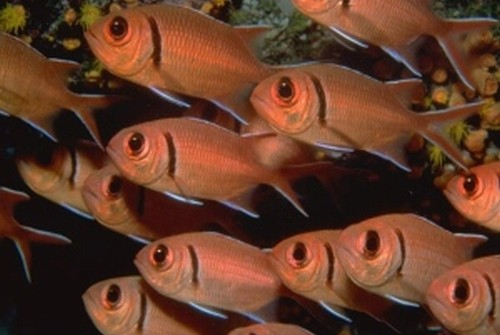
\includegraphics[width=20cm,trim={0 5cm 0 5cm},clip]{../output/fishes.jpg}}
  \caption{H αρχική εικόνα και τα KeyPoints επί της ασπρόμαυρης}
\end{figure}


\subsection{sunflowers.jpg}
\begin{figure}[H]
  \centerline{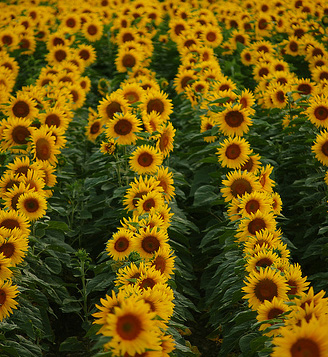
\includegraphics[width=20cm,trim={0 3cm 0 3cm},clip]{../output/sunflowers.jpg}}
  \caption{H αρχική εικόνα και τα KeyPoints επί της ασπρόμαυρης}
\end{figure}

\subsection{otter.jpg}
\begin{figure}[H]
  \centerline{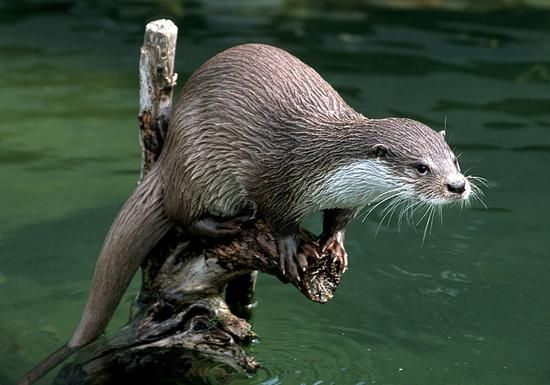
\includegraphics[width=20cm,trim={0 5cm 0 5cm},clip]{../output/otter.jpg}}
  \caption{H αρχική εικόνα και τα KeyPoints επί της ασπρόμαυρης}
\end{figure}

\subsection{plumeria.jpg}
\begin{figure}[H]
  \centerline{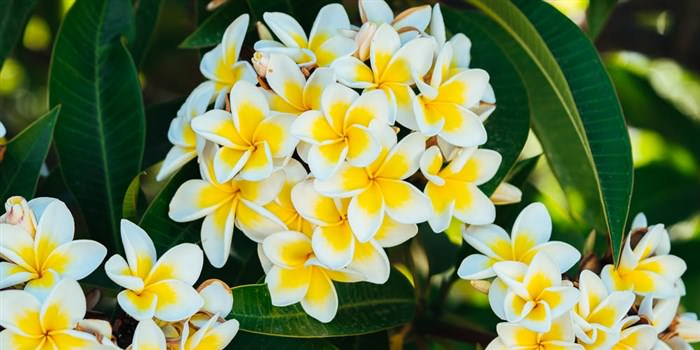
\includegraphics[width=24cm,trim={0 6cm 0 6cm},clip]{../output/plumeria.jpg}}
  \caption{H αρχική εικόνα και τα KeyPoints επί της ασπρόμαυρης}
\end{figure}

\section{Συμπεράσματα}

Όπως φαίνεται στις παραπάνω εικόνες, ο αλγόριθμος κάνει αρκετά καλή δουλεια στην αναγνώριση των KeyPoints.
Ενδιαφέρον έχει να αναλύσει κανείς τις ακτίνες των κύκλων. Βλέπουμε πως τα σημαντικά points of interest
(απότομες εναλλαγές σε χρώμα, edges και lines) συνήθως αναπαρηστούνται με μικρούς κύκλους.
Οι κύκλοι μεγάλης ακτίνας είναι συνήθως σε (μεγαλύτερες) περιοχές με σταθερό χρώμα. Δηλαδή, αναγνωρίστηκαν ως
KeyPoints σε μεγάλη οκτάβα και scale. Aυτό γίνεται κατανοητό παρατηρώντας το Scale-Space, καθώς με το
blur και την αρκετά μικρή διάσταση (περίπου 20x30 pixel) είναι πιο πιθανό να αναγνωριστούν
οι εναλλαγές σε μεγαλύτερες περιοχές.

\subsection{Σύγκριση με γνωστούς αλγορίθμους}
Τέλος βλέπουμε πως ο προτεινόμενος αλγόριθμος κάνει αρκετά καλή δουλειά, αφού με τις ίδιες ρυθμίσεις για
octaves και layers, είμαστε αρκετά κοντά στο αποτέλεσμα του \texttt{SURF} και μάλιστα θα μπορούσε κανείς
να πει πως ο δεύτερος έχει και μερικά στοιχεία false-positive, οπότε θα ήταν θεμητό να χρησιμοποιηθεί με
κάποιον επιπλέον ταξινομητή για να χρησιμοποιήσει τα ``χρήσιμα'' keypoints.

\begin{figure}[H]
  \centerline{\includegraphics[width=18cm,clip]{../output/compare.jpg}}
  \caption{Παρατηρήστε τις μαύρες περιοχές και την ύπαρξη false-positive από τον SURF}
\end{figure}

Κλείνοντας, να αναφέρουμε πως μπορεί κανεις να συμπεράνει, κάνοντας reverse engineering, ότι
και ο αλγόριθμος SURF υλοποιεί resize του επιπέδου των scale κι αυτός είναι ο λόγος που αναγνωρίζονται
kaypoints στα ``σκοτεινά'' σημεία της εικόνας, καθώς το low contrast rejection δε λειτουργεί στις
πολύ μικρές εικόνες.

\begin{figure}[H]
  \centerline{\includegraphics[width=18cm,clip]{../output/fishes_efficient_like_SURF.jpg}}
  \caption{Παρατηρήστε την ύπαρξη false-positive, όπως στο αποτέλεσμα του SURF}
\end{figure}

Τέλος, βλέπουμε πως η efficient μέθοδος τρέχει \textbf{περίπου 10 φορές πιο γρήγορα}.

\vspace{1cm}
\textit{Σημείωση:} έχει υλοποιηθεί και η efficient μέθοδος με upsampling του scale space
έτσι ώστε να έχουν όλες οι κλίμακες το μέγεθος της οκτάβας. Με αυτό τον τρόπο δε χρειάζεται
παραμετροποίηση η \texttt{generateExtrema} και αλλάζει μόνο ο χρόνος εκτέλεσης της \texttt{generateScaleSpace}.
Παρ` όλ' αυτά η χρονική διαφορά δεν απέχει από την inefficient μέθοδο. Το rescale των γειτονικών
scale στην \texttt{generateExtrema} δεν έγινε, αλλά δεν θα άλλαζε και πολύ τα αποτελέσματα καθως αν το
\texttt{sample\_point} είναι extrema θα συνέχιζε να είναι, δηλαδή τα σωστά KeyPoints τα θα αναγνωριζόταν.
Αυτός είναι και ο λόγος που υπάρχουν false positive (το οτι χωρίς resampling αναζητούμε σε μεγαλύτερες
περιοχές που δεν θα έπρεπε).

\vspace{4cm}
\subsection{Κώδικας}
\matlabscript{../src/generateLoGfilters}{Η δημιουργία φίλτρων.}
\matlabscript{../src/generateScaleSpace}{Η ανάλυση.}
\matlabscript{../src/generateExtrema}{Η αναγνώρηση.}
\matlabscript{../src/reduce}{To downsample.}
\matlabscript{../src/main}{Πρόγραμμα οδηγός.}
% \matlabscript{../src/show\_all\_circles}{Προβολή keypoint.}

Τέλος ο κώδικας για τον SURF:
\lstinputlisting[language=C++]{../src/openCV_cpp_SURF/main.cpp}{OpenCV-4, GNU/Linux compatible Makefile included}

\begin{thebibliography}{2}

\bibitem{lowe}
DAVID G. LOWE, Distinctive Image Features from Scale-Invariant Keypoints,
\url{https://www.cs.ubc.ca/~lowe/papers/ijcv04.pdf}

\bibitem{otero}
Ives Rey Otero, and Mauricio Delbracio, Anatomy of the SIFT Method, Image Processing On Line, 4 (2014), pp. 370–396.
\url{https://doi.org/10.5201/ipol.2014.82}

\end{thebibliography}

\end{document}
